%
% @author Kalvin Döge
%


\section{Stand der Wissenschaft}\label{sec:state-of-science}

Die Idee, Lichtsignalanlagen an Kreuzungen mit einer vorherbestimmten Steuerung zu verwalten, ist aber nicht keine neue.
Mehrere Forscher haben bereits Lösungen über künstliche Intelligenzen, durch Fokussierung auf die Fahrradfahrer oder zeitlicher Abstimmung von den Lichtsignalphasen gefunden.

\textbf{Ye Zheng, Ding Ma, Fengying Jin und Zhigang Zhao:}
\textit{Intelligent Traffic Signal Control Based on Reinforcement Learning with State Reduction for Smart Cities}

In dem Forschungsbeitrag von Li Kuang und andere aus dem Jahr 2019, widmen sich die vier Autoren auf eine Lösung mithilfe eines Q-Learning-Algorithmus.
Dadurch, dass die Infrastruktur der Straßen nicht weiter ausgebaut werden kann in urbanem Verkehr, bleibt nur noch das Auflösen von Staus bei Lichtsignalschaltung und Kreuzungen\cite{Zheng2019}, weshalb sie sich mit dieser Arbeit an den Ansatz mit einer künstlichen Intelligenz setzten.

Die Aufgabe von bis entwickelten Echtzeitlösungsansätzen, so Zheng und andere, sind vier Kategorien zuzuordnen:
Feste Zeitschaltungen mit Anpassungen je Tageszeit, vorhersagende Signalschaltung aufgrund von Eingabedaten aus vergangenem oder aktuellem Verkehrsfluss, Betätigungssignalschaltung mit der bei Aktivierung von Sensoren Grün- oder Rotphasen verlängert werden und die Adaptivschaltung, die mit Sensoren und mit Algorithmen den Verkehr zum Zeitpunkt des Eintretens die Schaltungen verändern\cite{Zheng2019}.

Ihr Ansatz mit der künstlichen Intelligenz fällt unter eine neue Lösungsstrategie, mit der sie Lichtsignalphasen bei einzelnen Kreuzungen über das verstärkte Lernen abstimmen wollen\cite{Zheng2019}.
Beispielsweise sind gegenüberliegende, geradlinig gerichtete Straßenspuren, wie in der Grafik~\ref{fig:kuang-lanes} bei zum Beispiel den Spuren 6 und 2 zu sehen ist, miteinander verknüpfbar als eine Lichtsignalphase, da sie keine Überkreuzung ihrer Fahrbahn haben.
Um diese Phaseneinteilung für die künstliche Intelligenz vorzubereiten, sollen die einzelnen Fahrbahnen in Kombination mit Fahrzeugdaten in Gruppen unterteilt werden\cite{Zheng2019}.

\begin{figure}[h]
    \centering
    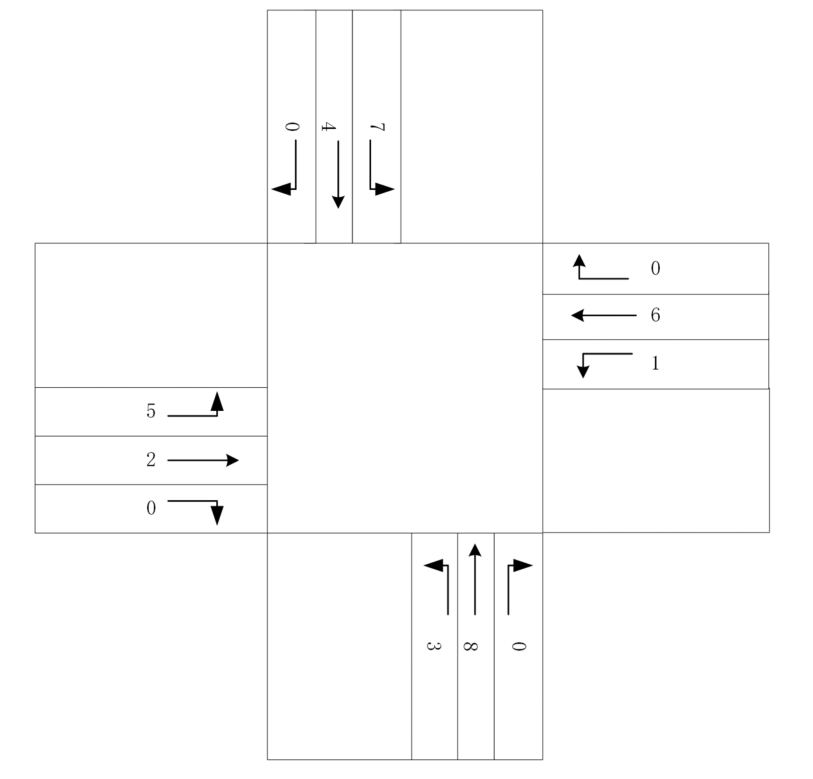
\includegraphics[width=0.75\textwidth]{kuang-lanes}~\caption{Das von Kuang und andere bei einer 3-spurigen Kreuzung dargelegte 8-Phasen Modell~\cite{Zheng2019}}
    \label{fig:kuang-lanes}
\end{figure}

Damit ließe sich der Algorithmus dann noch weiter verfeinern, als dass sie seltene oder fast nie auftretende Szenarien aus der Menge möglicher Zustände entfernen und sich nur die einzelnen Zahlen als Eingabe erhalten muss, nicht die gesamte Struktur der Kreuzung.

Im Folgenden gehen sie auf weitere Arbeiten ein, die eine andere Größenskalierungen als sie vorgenommen haben, bevor sie dann auf die genaue Implementation des Straßenmodells und dem Lernen beziehungsweise Trainieren der künstlichen Intelligenz eingehen.

Ein Problem bei der Phaseneinteilung ist aber, dass sie bei einzelnen Kreuzungen annahmen, dass jede Kreuzung je 3 eingehende Straßen hat, die in die Kreuzung münden.
Auch wenn die Stauzonen meist große Kreuzungen sind, so haben Städte auch Lichtsignalschaltungen verschiedene Kreuzungen mit mehr als nur 3 oder teilweise auch nur 2 Spuren, sodass ein Q-Learning-Algorithmus nicht mit solchen Szenarien umgehen kann und bei anderen Kreuzungen von vorne konzipiert und trainiert werden muss.

Dennoch ist die Einteilung der verschiedenen Lösungsansätze ein wichtiger Aspekt, der auch in dieser Arbeit Relevanz hat, explizit der erste Typ, die feststehende Zeitschaltung.


\textbf{Valentina Kurtc und Martin Treiber:}
\textit{Simulating bicycle traffic by the intelligent-driver model-Reproducing the traffic-wave characteristics observed in a bicycle-following experiment}

Der Forschungsbeitrag von Kurtc und Treiber aus dem Jahr 2020 untersucht die Hypothese, dass sich die Bewegungsdynamik des Fahrzeugverkehrs qualitativ nicht unterscheidet von dem Fahrradverkehr, indem sie die Qualität eines Fahrzeugmodells beziehungsweise Pkw-Modells ebenso für Fahrräder nutzen können.
Dies beweisen sie mit einem ,,Intelligent Driver Model``\cite{Kurtc2020}, einem mikroskopischen Modell für Autos, und vergleichen dessen Qualität der Kalibrierung und Vorhersagefähigkeit dann mit dem ,,Necessary Decelaration Model``\cite{Kurtc2020}, einem mikroskopischen Fahrradmodell.

Im Folgenden gehen Kurtc und andere darauf ein, wie sie eine Vergleichsbasis über die Formel herstellen und das anhand der Beschleunigungsfunktionen aus den Modellen aufbauen, um dann ein Kreisverkehrsszenario mit einem Fahrraddatenset zu simulieren und die berechneten Ergebnisse zu vergleichen.

\begin{figure}[h]
    \centering
    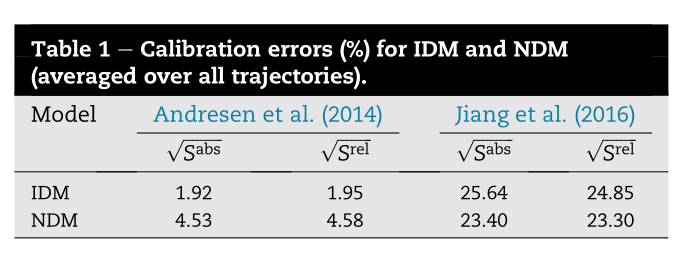
\includegraphics[width=0.75\textwidth]{kurtc2020}~\caption{die von Kurtc und Treiber berechneten, durchschnittlichen Kalbirierungsfehler der beiden Modelle in \%~\cite{Kurtc2020}}
    \label{fig:kurtc2020}
\end{figure}

Das Ergebnis aus der Grafik~\ref{fig:kurtc2020} zeigt, dass die Unterschiede der Modelle beim Nutzen von Fahrraddaten klein sind, als dass sie keinen großen Effekt auf die Simulationen haben.

Aus Kurtc und Treibers Forschungsarbeit lässt sich für diese Simulation also ableiten, dass Agenten, die auf der Straße fahren und Modalitäten wechseln, sowohl mit den Bewegungsmodellen von Fahrrad und Auto simuliert werden können, ohne an Akkuratheit einbüßen zu müssen.


\textbf{Saif Islam Bouderba und Najem Moussa:}
\textit{Reinforcement Learning (Q-LEARNING) traffic light controller within intersection traffic system}

In dem Thesenpapier von Bouderba und Moussa aus dem Jahr 2020 wird eine ähnliche Hypothese wie die von Kuang und andere untersucht.
Sie untersuchen die Effektivität von drei Lösungsansätzen für ihr zelluläres Automatenmodell sind:
Bei dem ersten Experiment simulieren sie einen einfachen, synchronisierten Ablauf der Lichtsignalschaltungen, beim Zweiten einen Ansatz einer ,,Grünen Welle``-Schaltung mit aufeinanderfolgenden Ampeln und beim Dritten eine durch Q-Learning-Algorithmus gesteuerte Kreuzungen~\cite{Bouderba2019}.

Ihr Automatenmodel besteht dabei aus einer Matrix an Kreuzungen, die alle von der Position her mit ihren umliegenden Nachbarn über eine zweispurige Straße verbunden sind:

\[N \times N = 4\]

Jede Kreuzung hat also vier Eingangs- und Ausgangspunkte sowie eine Lichtsignalanlage, die mit je einer Lösungsstrategie pro Experiment gesteuert wird.
Zudem ist die Simulationsumgebung aufgeteilt in Zellen, auf denen sich die Agenten entlangbewegen und zu den Kreuzungen gelangen\cite{Bouderba2019}.

\begin{figure}[h]
    \centering
    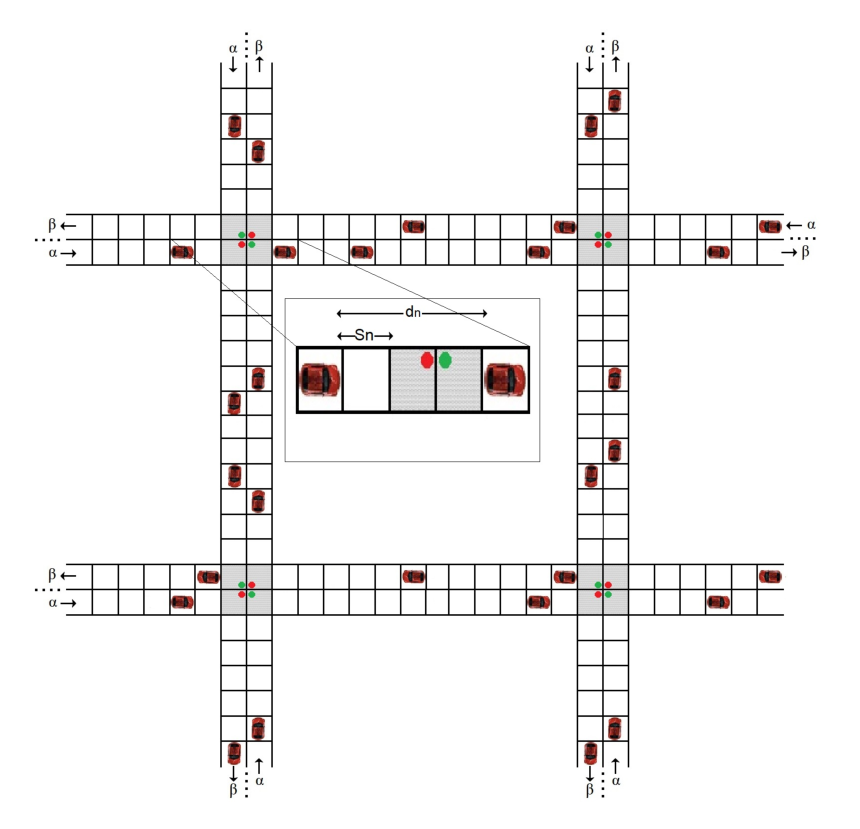
\includegraphics[width=0.75\textwidth]{bouderba-cells-model}~\caption{Eine Momentaufnahme aus dem zellulären Automatenmodell~\cite{Bouderba2019}}
    \label{fig:bouderba-cells-model}
\end{figure}

Mit dem Modell~\ref{fig:bouderba-cells-model} als Simulationsgrundlage erläutern Bouderba und Moussa die Lösungsstrategien.
Die grüne Welle Synchronisation erfolgt über eine Verschiebung der aktuellen, internen Zeituhr von umliegenden Lichtsignalen, während der Q-Learning-Alhorithmus trainiert wird, um eine passende Schaltung selbst zu erlernen.

\begin{figure}[h]
    \centering
    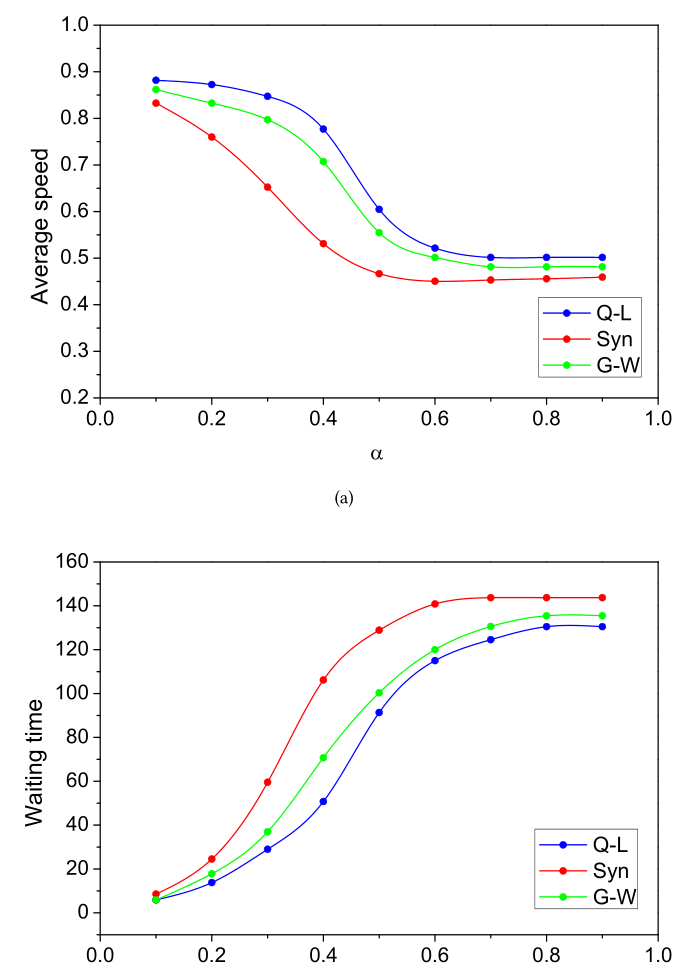
\includegraphics[width=0.5\textwidth]{bouderba-results}~\caption{Die durchschnittliche Geschwindigkeit und Wartezeit nach Durchführunge~\cite{Bouderba2019}}
    \label{fig:bouderba-result-graph}
\end{figure}


Die Resultate in Geschwindigkeit und Wartezeit pro Eingriffsrate aus Grafik~\ref{fig:bouderba-result-graph} zeigen auf, dass der einfache, synchronisierte Ansatz am schlechtesten von allen drei Algorithmen abschneidet.
Die durchschnittliche Wartezeit ist höher als die von dem Q-Learning-Algorithmus und der grünen Welle, genauso wie die durchschnittlichen Geschwindigkeitsmessungen niedriger ausfällt als bei den anderen beiden Ansätzen.

Auch wenn die Grüne-Welle-Schaltung in den Experimenten besser abschnitt, so ist dieser Ansatz nicht der dieser Arbeit.
Der Unterschied besteht darin, dass in Bouderba und Moussas Forschungsarbeit die Ampelphasenlängen auf ihrer Distanz basierend verlängert wurden.
Dies soll in dieser Arbeit aber durch eine insgesamt geltende Phasenschaltung ersetzt werden, da Agenten hier mehr als nur Geschwindigkeit erhöhen und senken können.
Sie können zum Beispiel kleine Veränderungen an Routen unternehmen, sodass sie nicht auf der Straße, sondern auf Fahrradwegen vorbeifahren und Lichtsignalschaltungen ignorieren.
Diese Bewegungsfreiheit der Agenten ist in dem Modell von Bouderba und Moussa nicht gegeben, weshalb die Forschungsarbeit nur als Motivation für die Verbesserungsmöglichkeiten einer grünen Welle angesehen werden kann.


\textbf{Katharina Mulack:}
\textit{Multiagenten Simulation von Fahrradfahrern im Kontext urbaner Verkehrsdynamik}

Die Masterarbeit von Katharina Mulack aus dem Jahr 2020 basiert ebenso auf dem MARS-Framework und ergänzt die bis zu dem Zeitpunkt der Arbeit in dem Framework fehlenden Fahrradfahrer.
Dabei fokussiert sich die Arbeit auf die detailreiche Rekonstruierung von Fahrradfahrern mit einem eigenen Bewegungsmodell, Statistiken über Eigenschaften von Fahrrädern und deren Interaktion mit der Umgebung\cite{Mulack2020}.
Bei den Verkehrsflussmodellen, einem Kernaspekt der Forschungsarbeit, wird insbesondere auf vier unterschiedliche Modellierungskonzepte eingegangen, die sich in der Feinheit der Simulationsmodelle unterscheiden:

Makroskopische Flussmodelle, die bei Simulationen sich mit dem allgemeinen Verlauf beschäftigen und die Details wie die Simulation einzelner Fahrzeuge nicht simulieren, um das Gesamtverhalten und ihr Effekt der Bewegung zu beobachten\cite{Mulack2020}.

Mikroskopische Modelle wiederum dienen der detaillierteren Simulation und beziehen individuelle Verhaltensweisen von Agenten mit der Umwelt oder anderen Agenten ein\cite{Mulack2020}.

Submikroskopische Modelle wiederum sind noch spezifischer und simulieren sogar Beziehungen zwischen Agenten und Entitäten, um den Detailgrad der echten Welt zu imitieren\cite{Mulack2020}.

Zuletzt wird noch das Mesoskopische Modell genannt, welches eine Mischung aus Makro- und Mikroskopmodell ist.
Bei diesem werden sowohl über große Distanzen und Gesamtverhalten angeschaut werden, dennoch aber die einzelnen Agenten oder Entitäten diese große Veranschaulichung ausmachen\cite{Mulack2020}.

Im Folgenden untersucht Mulacks Masterarbeit die Verkehrsflussmodelle und Statistiken über Fahrräder und implementiert sie zusammen mit neuen Umwelteinflüssen, den Lichtsignalanlagen.

Mulacks Forschungsarbeit selbst befasst sich mit einem hohen Detailgrad und zwischenagentlichen Beziehung bei den Fahrradfahrern, während sich diese Arbeit hier eher mit einem gemischten, mesoskopischen Simulationsmodell beschäftigt.
Zwar wird in dieser Arbeit ebenfalls auf einzelne Agenten benutzt, die mit ihrer Umwelt und den Entscheidungen andere Agenten beeinflussen, aber ist die generelle Stau- und Warteschlangenbildung wichtiger für die Ergebnisse.

Auch beschäftigt sich die Arbeit mehr mit dem Verhalten der Fahrradfahrer selbst innerhalb des MARS-Frameworks, nicht mit der Entwicklung einer optimalen Lichtsignalschaltung.
Dies macht diese Masterarbeit zu einer geeigneten Quelle für detailreiche Verhaltensweisen von Fahrrädern, weniger aber zu einem vergleichbaren Ansatz für diese Arbeit.


\textbf{Thomas Clemen, Nima Ahmady-Moghaddam, Ulfia A. Lenfers, Florian Ocker, Daniel Osterholz und Jonathan Ströbele:}
\textit{Multi-Agent Systems and Digital Twins for Smarter Cities}

In der Forschungsarbeit aus dem Jahr 2021 beschäftigen sich Clemen und andere mit dem ,,Internet of Things``, fortan als IoT abgekürzt, welches eine Großzahl an (Echtzeit-) Daten über die Stadt Hamburg via Sensoren anbietet, und entwickeln dazu ein digitales Zwillingsmodell der Stadt selbst, zur Überführung der Daten in das MARS-Framework.
Im Zentrum dabei steht nicht nur die Nutzungsermöglichung der IoT-Daten, sondern ebenfalls die Frage: Wie baut werden ort- und zeitlich gebundene Daten in ein Echtzeitmodell integriert, in der sich die Simulationen und Experimente anschaulich darstellen und kontrollieren lassen sollen~\cite{Clemen2021}?

Ihr Lösungsweg: Das Herunterbrechen der Akteure in der echten Welt auf Agenten und Entitäten, die damit als eine digitale Zwillingsinstanz~\cite{Clemen2021} fungieren und das Verhalten der Akteure oder Simulationsflächen imitieren.
Dabei wird zudem noch ein Fokus darauf gelegt, zwischen passiven, aktiven und interagierbaren Zwillingsinstanzen zu unterscheiden, da der Verhaltens- und Implementationsaufwand durch die Entscheid- und Bewegungsfreiheit steigt.
Entsprechend entscheiden sie sich, in ihrer Forschung vorerst die Echtzeitdaten nur bei passiven Zwillingsinstanzen zu implementieren.
Als Grundlage dafür wird das SmartOpenHamburg-Projekt genommen, was bereits die physische Repräsentation der Stadt sowie eine Reihe der städtischen Modalitäten implementiert hat, und erweitern dieses um den Zugang zu den IoT-Daten~\cite{Clemen2021}.

Dadurch, dass in der Forschungsarbeit von Clemen und andere nur die passiven, digitalen Zwillinge mit Daten angereichert werden, fehlt für die Arbeit hier die Echtzeitdaten von Lichtsignalschaltungen sowie einem Echtzeitverkehrssensor.
Da in der Arbeit von diesem Papier hier sich auf den Verkehrsfluss und explizit auf die Simulation einzelner Agenten fokussiert wird, müssen diese aktiven Agenten sein, die Entscheidungen über Modalitäten, Wege und Interaktion mit Entitäten unternehmen.
Damit würden sie unter die interagierbaren, digitalen Zwillinge fallen, die mit Eingabedaten bestückt werden müssten und sind entsprechend mit einem großen Mehraufwand beim Implementieren verbunden.

Entsprechend ist die Forschung der Arbeit von Clemen und andere zwar eine gute Grundlage für zukünftige Ausblicke dieser Arbeit, sollten Echtzeitdaten bereitgestellt werden für aktuellen Verkehr an Lichtsignalanlagen oder generell auf Straßen.
Jedoch ist der Nutzen für diese Arbeit beschränkt auf das SmartOpenHamburg-Projekt, dass die Grundlagen zur agentenbasierten Simulation bereits bereitstellt.


\textbf{Daniel Glake, Fabian Panse, Norbert Ritter, Thomas Clemen und Ulfia Lenfers:}
\textit{Data Management in Multi-Agent Simulation Systems}

Daniel Glake und andere beschäftigten sich im Jahr 2021 in ihrem Forschungsbeitrag mit den Problemen des Einbauens von unterschiedlichen Daten in einem sehr groß skalierten Simulationsszenario und präsentieren dabei Lösungen für die Herausforderungen mithilfe des MARS-Frameworks.
Dabei fokussieren sie sich auf fünf großen Eingabedatenkategorien, die in der MARs-Simulationsumgebung eingebaut werden und mit großskalierten Projekten zu Herausforderungen kommen können:
\begin{itemize}
    \item Eingabedaten für Simulationen, die zum Beispiel bei einem Ortstransfer zu Kompabilitätskomplikationen führen, wie etwa mit geografischen Karten, den lokalen Infrastrukturnetzwerken oder weitere, nicht-ortsgebundene Daten wie zeitliche Busfahrpläne~\cite{Glake2021}.
    \item Ausgabedaten von großen Simulationen, die beim Simulieren eine Großzahlan Agenten und Entitäten nutzen, blockieren beziehungsweise verzögern beim Exportieren von Zwischenständen die aktive Simulation deutlich und schränken damit die Fähigkeit diese in Echtzeit zu analysieren ein~\cite{Glake2021}.
    \item Eingabedaten über Streams werden beim Vorhersagen von Simulationszuständen, wie etwa den Agentattributen oder Umweltinformationen, immer ungenauer je weiter in die Zukunft berechnet wird.~Dafür bieten Schnittstellen und angebundenen Systeme Möglichkeiten zum vermindern dieser Ungenauigkeit.~Das Korrigieren benötigen aber dennoch bei einer großen Anzahl von Agenten einem Moment zum Überreichen, was zeitlich ebenfalls zu Verzögerungen führen und auch die Echtzeitanalysefähigkeit erschwert~\cite{Glake2021}.
    \item Bei Schnittstellen für räumlich-zeitliche Abfragen wird stets der jeweilige Raum benötigt und zum Beispiel in MARS als Polygon angegeben.~Operationen wie ,,beinhält``, ,,überlappt`` oder ,,ist adjazent von`` sind dabei häufig genutzt, was bei einer Vielzahl von Agenten, die dies gleichzeitig durchführen und sich dabei bewegen, zu zeitlichen sowie geographischen Unterschieden führt~\cite{Glake2021}.
    \item Beim Planen dieser räumlich-zeitlichen Abfragen, wie das System die echte Welt auf die Modellrepräsentation abzubilden hat, darf die Migrationszeit nicht die Datenverarbeitungszeit überschreiten, damit es nicht zu Inkonsistenzen in der Simulation führt.~Strategien, die das verhindern, sind aber nur Annäherungen, da die Optimierung der Migrationszeit einem NP-Problem entspricht und somit nicht mit einer konstanten Anzahl an Operationen berechnet werden kann~\cite{Glake2021}.
\end{itemize}

Danach gehen Glake und andere genauer darauf ein, wie sie diese Problematiken im MARS-Framework mit Lösungsansätzen vermindert oder gelöst bekommen haben.
Für diese Arbeit hat die Forschungsarbeit von Glake und andere aber keinen relevanten Bezug:
Das System hier ist kein Echtzeitsystem auf einem großskalierten Bereich.
Der Simulationsraum beschränkt sich auf die Binnen- und Außenaslter und zur Ergebnissermittlung genügt es bereits, wenn die Simulation nebenbei berechnet wird.
Eine Verzögerung aufgrund von groß skalierten Bereichen oder zu vielen Agenten affektiert nicht die Korrektheit des Systems und ist sich also nicht von den kategorisierten Problemen affektiert.

Dennoch wären für zukünftige Arbeiten das Papier von Glake und andere ein guter Ansatz, um Echtzeitdaten mit der gesamten Stadt Hamburg zu verbinden und damit den gesamten Raum zu simulieren, nicht nur wie hier um die Binnen- und Außenalster.


\textbf{Ulfia A. Lenfers, Nima Ahmady-Moghaddam, Daniel Glake, Florian Ocker, Daniel Osterholz, Jonathan Ströbele und Thomas Clemen:}
\textit{Improving Model Predictions—Integration of Real-Time Sensor Data into a Running Simulation of an Agent-Based Model}

In einem weiteren Forschungsartikel über das MARS-Framework im SmartOpenHamburg-Projekt des Jahres 2021 beschäftigen sich Ulfia A. Lenfers und andere mit der Verbesserung der Einbindungsimplementation von Echtzeitdaten und zeigen das Potenzial anhand von Fahrradverleihstationen, wie mit der Modellierung und Daten genauere Vorhersagungen zu Fahrradverleihs getroffen werden können.

\begin{figure}[h]
    \centering
    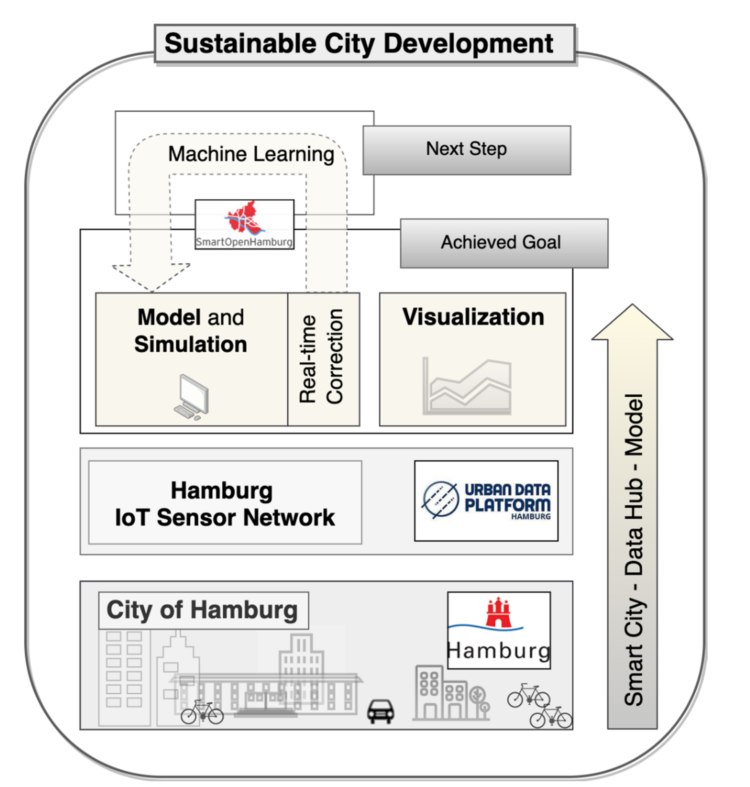
\includegraphics[width=0.75\textwidth]{lenfers-workflow}~\caption{Beispielworkflow, wie Daten aus den Sesnsoren und von der Stadt Hamburg in ein abstraktes Simulationsmodell eingebaut werden~\cite{Lenfers-MP-2021}}
    \label{fig:lenfers-workflow-sensors}
\end{figure}

Wie aus dem Workflow von~\ref{fig:lenfers-workflow-sensors} zu entnehmen ist, fokussiert sich der Kern der Arbeit aus dem Zusammenspiel von Datenfluss des Smart-City-Data-Hub und die Dateneinbindung von Fahrradverleihstationen in die SmartOpenHamburg-Komponente.
Echtzeitdaten werden bei ihrer Implementation von der ,,Smart City`` über ein zeitlichen Vektor-Layer in die Simulation konstant eingelesen und anhand ihrer Lebenszeit entsprechend simuliert\cite{Lenfers-MP-2021}.
Die Daten selbst werden dabei über eine URI von den externen Endpunkten abgefragt und mit zusätzlichen Argumenten auf die relevanten Daten reduziert~.
Mit diesem Datenstrom werden die derzeitigen Zustände der Fahrradverleihstationen abgefragt und in die Simulation eingebaut, wie viele Fahrräder derzeit aktuell aktiv genutzt werden und wie viele Agenten in der Simulation agieren\cite{Lenfers-MP-2021}.

Der Forschungsbeitrag von Lenfers und andere ist aber, wie bei der vorherigen, für diese Arbeit nur begrenzt relevant: Die statische Implementation von Fahrradverleihstationen ist relevant, da Verkehrsteilenhmer an den Stationen sich ein Fahrrad leihen können, doch ist dabei kein Echtzeitstrom vonnöten und passiert passiv nebenbei.

Dennoch bietet die Arbeit Anknüpfmöglichkeit, sollten relevanten Echtzeitdaten von der Stadt Hamburg zum Verkehr oder zu Lichtsignalanlagen über die nächste Zeit aufkommen und damit den Kern einer anderen Arbeit darstellen.


\textbf{Daniel Glake, Fabian Panse, Norbert Ritter, Thomas Clemen und Ulfia Lenfers:}
\textit{Incorporating Multi-Modal Travel Planning into an Agent-Based Model: A Case Study at the Train Station Kellinghusenstraße in Hamburg}

Der Forschungsartikel von Lenfers und andere aus dem Jahr 2021 erweitert ebenfalls das MARS-Framework und das SmartOpenHamburg-Projekt um nachhaltige Modalitäten wie die mietbaren Äquivalente zu Pkws und Fahrrädern oder das Zu-Fuß-Gehen.
Dabei untersuchen sie, wie effizient das Wechseln der Modalitäten in einem Beispielszenario ist und ob die Optimierungsstrategien hinsichtlich der Klimaneutralität, aus finanziellen Gründen oder persönlichen Präferenzen korrekt annähern~\cite{Lenfers-MMT-2021}.

Das Beispielszenario, welches sie zur Demonstrierung der implementierten Modalitäten verwenden, umfasst dabei die Bahnhofsstation Kelinghusenstraße in Hamburg, von der aus die Agenten mit den Modalitäten in einem Kreis-Bereich zu ihrem Ziel gelangen können.

\begin{figure}[h]
    \centering
    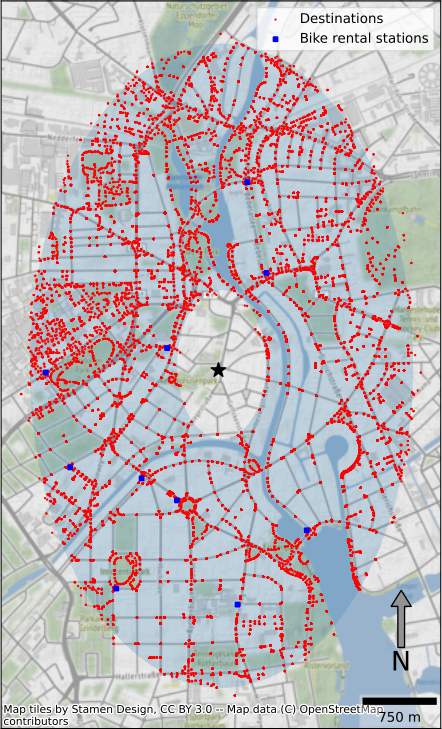
\includegraphics[width=0.75\textwidth]{lenfers-kelinghusen}~\caption{Karte der Fahrradverleihstationen, mit dem Simulationsbereich der Agenten hellblau hinterlegt, den Interessenspunkten rot markiert und Fahrradverleihstation als blaue Markierungen~\cite{Lenfers-MMT-2021}}
    \label{fig:lenfers-kelinghusen-area}
\end{figure}

Auf dem Weg zu ihrem Endziel innerhalb des simulierbaren Bereichs aus~\ref{fig:lenfers-kelinghusen-area} kommen manche Agenten durch angestrebtes Nutzen der Modalitäten erst zur nächsten Fahrrad- oder Pkwverleihstation, bevor sie ihre Reise zum Interessenspunkt fortsetzen können.
Dieses angestrebte Nutzen wird in den Eingabedaten durch zum Beispiel die Variablen ,,hasCar`` und ,,usesBikeAndRide`` versinnbildlicht, wie hoch die Wahrscheinlichkeit zum Nutzen oder Besitzen einer eigenen oder gemieteten Modalität ist~\cite{Lenfers-MMT-2021}.

Auf den implementierten Modalitäten und Verleihstationen aus der Forschungsarbeit von Lenfers und andere knüpft diese Arbeit hier an und untersucht nun mithilfe der Auswahl an Modalitäten eine mögliche Lichtsignalschaltung.
Damit bietet diese Arbeit eine sehr gute Grundlage, auf der nun aufgesetzt und das hier in dieser Arbeit beschriebenen Szenario aufgesetzt wird.
